
\documentclass[11pt,german,hideothersubsections]{beamer}

\usepackage{hyperref}
\usepackage{amsmath,nicefrac,booktabs,mathabx}
\usepackage{natbib}
\usepackage{url}
\usepackage{textpos}
\usepackage{listings}
\definecolor{Rblau}{rgb}{.3,.6,.9}

\lstset{language=R,
        basicstyle=\ttfamily\footnotesize,
        keywordstyle=\color{blue}\bfseries,
        identifierstyle=\color{Rblau},
        commentstyle=\color{gray},
        stringstyle=\color{green}\ttfamily,
        showstringspaces=false,
        frame=tb}



\bibpunct{(}{)}{;}{a}{,}{,}
\usepackage[english]{babel}
\usepackage[latin1]{inputenc}
\usepackage{helvet}
\usepackage{graphicx}
\usepackage{color}
\usepackage{multirow,dcolumn}
\usepackage{ragged2e}
\usepackage{xcolor}
\usepackage{colortbl}
\usepackage{tikz}
\usetikzlibrary{calc}
\usepackage{booktabs}
\colorlet{tablesubheadcolor}{gray!25}
\colorlet{tableheadcolor}{gray!40}
\colorlet{tablerowcolor}{gray!15.0}
\usetheme[english]{Gesis}
\setbeamertemplate{navigation symbols}{}
\setbeamertemplate{footline}[frame number]%{\hspace*{.2cm}\insertframenumber}
\setbeamerfont{caption}{size=\footnotesize}
\usefonttheme[onlylarge]{structuresmallcapsserif} % alte Schrift

\newcommand{\R}[1]{{\tt \color{blue}  #1}}
\newtheorem{thm}{Theorem}
\newtheorem{rem}{Bemerkung}
\newtheorem{lem}{Lemma}

\definecolor{hellgrau}{rgb}   {0.109375,  0.40625,   0.51953125}
\definecolor{dunkelgrau}{rgb} {0.009375,  0.30625,   0.41953125}
\definecolor{dunkelgrau2}{rgb}{0.009375,  0.20625,   0.31953125}
\definecolor{hellbraun}{rgb}  {0.9140625, 0.8984375, 0.8046875}
\definecolor{hellbraun2}{rgb} {.95,       0.9,       0.8}
\definecolor{alertred}{rgb}   {0.8515625, 0.3828125, 0.08984375}
\definecolor{orange}{rgb}{1,0.5,0}


\setbeamercolor{firstsecslide}{fg=white,bg=dunkelgrau}
\setbeamertemplate{blocks}[rounded][shadow=true]

\newcolumntype{d}[0]{D{,}{.}{6}}

\newenvironment{itemizeol}{\begin{itemize}[<+->]}{\end{itemize}}
\newenvironment{descriptionol}{\begin{description}[<+->]}{\end{description}}

\newcolumntype{V}[1]{%
  >{\RaggedRight\hspace{0pt}}p{#1}%
}

\newcommand{\emphred}[1]{\textcolor{alertred}{#1}}
\newcommand{\emphcol}[1]{\textcolor{dunkelgrau}{\slshape #1}}

\setcounter{tocdepth}{1}
\setbeamercolor*{section in toc}{fg=hellgrau}
\setbeamertemplate{bibliography item}[default]
\makeatother
\addtobeamertemplate{frametitle}{}{%
\begin{textblock*}{100mm}(.91\textwidth,-1cm)

\includegraphics[height=1cm,width=2cm]{../../graphs/logos/GESIS_Logo_kompakt_en.jpg}
\end{textblock*}}
\title[Day 1]{Tutorial: Sampling, Weighting and Estimation\\ \Large{Day 1} }
%\subtitle{Umgang am Beispiel von Telefonstichproben}

\author[M. Sand]{Stefan Zins, Matthias Sand\\ and Jan-Philipp Kolb\\ \vspace{.5cm} \footnotesize{GESIS - Leibniz Institute\\ for the Social Sciences}}
%\institute{\includegraphics[width=4.5cm]{GESIS_Logo_informell}}
\date[]{\color{dunkelgrau}\footnotesize%
\begin{minipage}{8cm}%
\begin{center}%
\scriptsize{
\textbf{GESIS Summer School}\\ \tiny{Cologne, Germany}%
}\\
\vspace{0.25cm}
\textbf{August 24th, 2015}%

\end{center}%
\end{minipage}}%


\usepackage{Sweave}
\begin{document}
\Sconcordance{concordance:Day1.tex:Day1.Rnw:%
1 99 1 1 0 3 1 1 7 53 1 1 5 6 0 1 1 6 0 1 2 25 1 1 2 1 0 1 1 6 0 1 2 6 %
1 1 2 1 0 1 1 5 0 1 1 5 0 1 1 6 0 1 2 6 1 1 2 1 0 2 1 6 0 1 1 5 0 1 1 5 %
0 1 1 6 0 1 2 7 1 1 2 1 0 1 1 15 0 1 1 8 0 1 2 7 1 1 2 1 0 1 1 9 0 1 1 %
6 0 1 2 3 1 1 2 6 0 1 1 5 0 1 1 5 0 1 1 6 0 1 2 84 1 1 2 1 0 2 1 4 0 1 %
2 5 1 1 2 5 0 1 2 26 1 1 2 1 0 1 1 1 2 1 0 1 3 1 0 1 2 2 1 12 0 1 2 5 1 %
1 2 12 0 1 1 7 0 1 1 6 0 1 2 8 1 1 2 1 0 5 1 11 0 1 1 6 0 1 2 4 1 1 3 2 %
0 3 1 4 0 1 2 3 1 1 2 1 0 3 1 1 2 1 0 1 1 3 0 1 2 3 1 1 2 4 0 1 2 1 6 1 %
7 2 2 4 0 1 2 24 1 1 2 4 0 1 2 66 1}

\maketitle


%%%%%%%%%%%%%%%%%%%%%%%%presentation%%%%%%%%%%%%%%%%%%%%%%%%%

\begin{frame}[fragile]{Why R?}
%\frametitle{\vspace{-.05cm}\begin{center}Why R?\end{center}}
\begin{itemize}
\item Open Source 
\vspace{.25cm}
\item You can work with several datasets at the same time
\vspace{.25cm}
\item You can create your own objects, functions and packages
\vspace{.25cm}
\item Over 5,000 packages contributed by users available on CRAN
\vspace{.25cm}
\item[$\rightarrow$] Rapid implementation of new (scientific) developments
\vspace{.25cm}
\item[$\rightarrow$] Quick development of new tools that fit the user's demand
\end{itemize}
\end{frame}
%%%%%%%%%%%%%%%%%%%%%%%%%%%%%%%%%%%%%%%%%%%%%%%%%%%%%%%%%%%%%%%%%%%
\begin{frame}[fragile]{Getting Started - Download R}
%\frametitle{\vspace{-.05cm}\begin{center}\footnotesize{Getting Started - Download R}\end{center}}
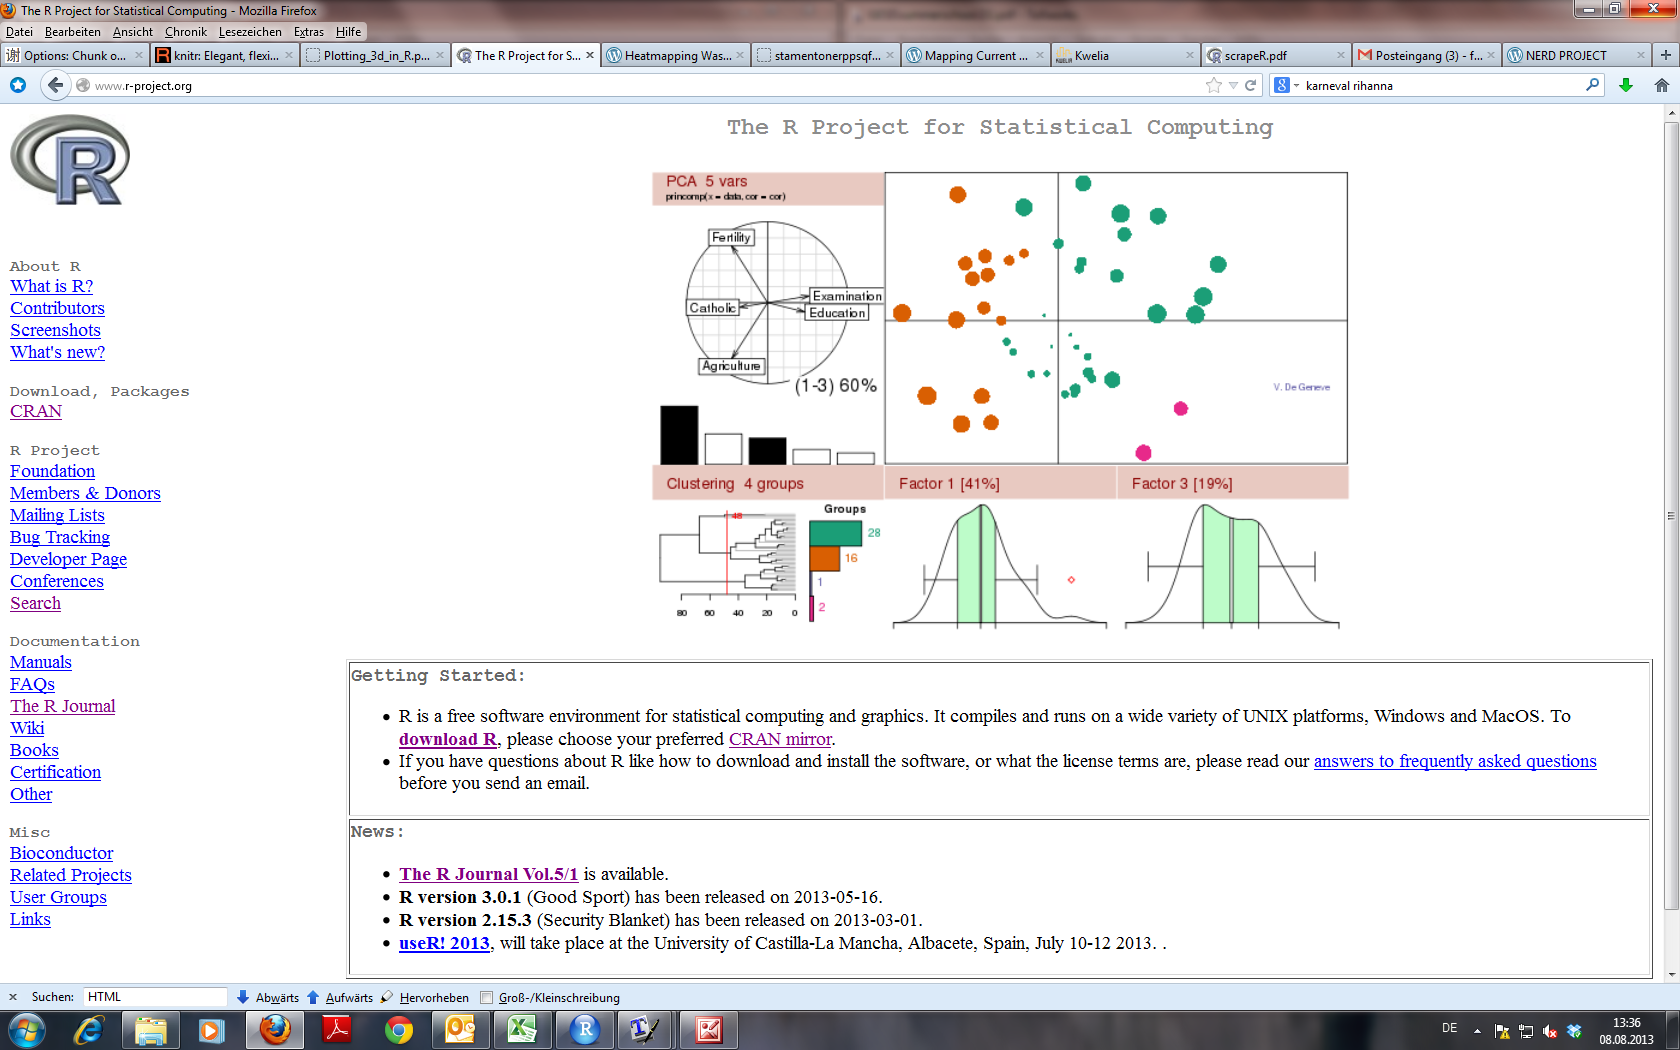
\includegraphics[width=\linewidth, height=6cm]{../figure/Rproject.png}
\vspace{.5cm}
\centering
\url{https://www.r-project.org}

\end{frame}
%%%%%%%%%%%%%%%%%%%%%%%%%%%%%%%%%%%%%%%%%%%%%%%%%%%%%%%%%%%%%%%%%%%
\begin{frame}[fragile]{R Basic}
%\frametitle{\vspace{-.05cm}\begin{center}\footnotesize{R Basic}\end{center}}
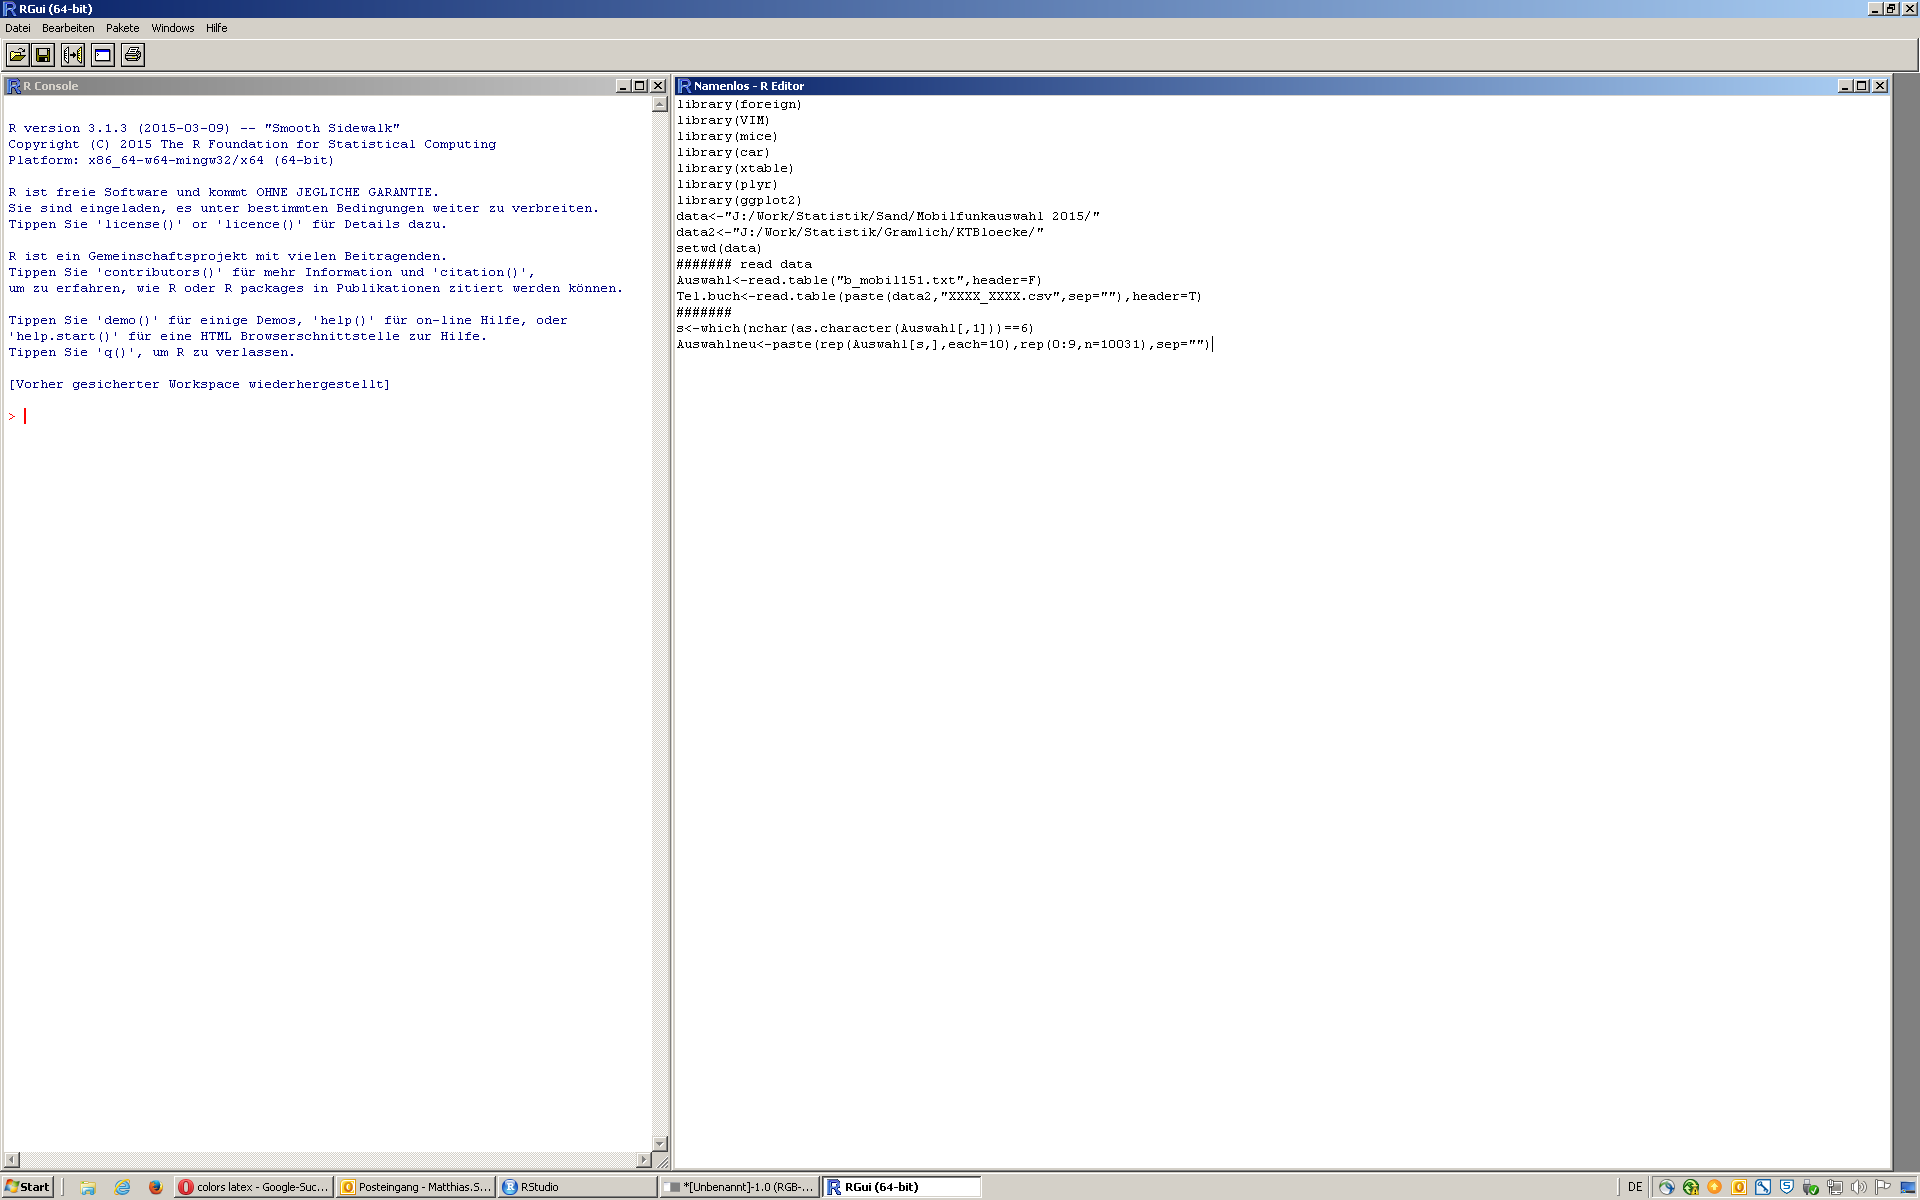
\includegraphics[width=\linewidth, height=6cm]{../figure/Ralt.png}
\begin{itemize}
\item most R-user prefer the graphical user interface (GUI) \href{https://www.rstudio.com}{\R{RStudio}}
\end{itemize}
\end{frame}
%%%%%%%%%%%%%%%%%%%%%%%%%%%%%%%%%%%%%%%%%%%%%%%%%%%%%%%%%%%%%%%%%%%%
\begin{frame}[fragile]{R Studio}
%\frametitle{\vspace{-.05cm}\begin{center}\footnotesize{R Studio}\end{center}}
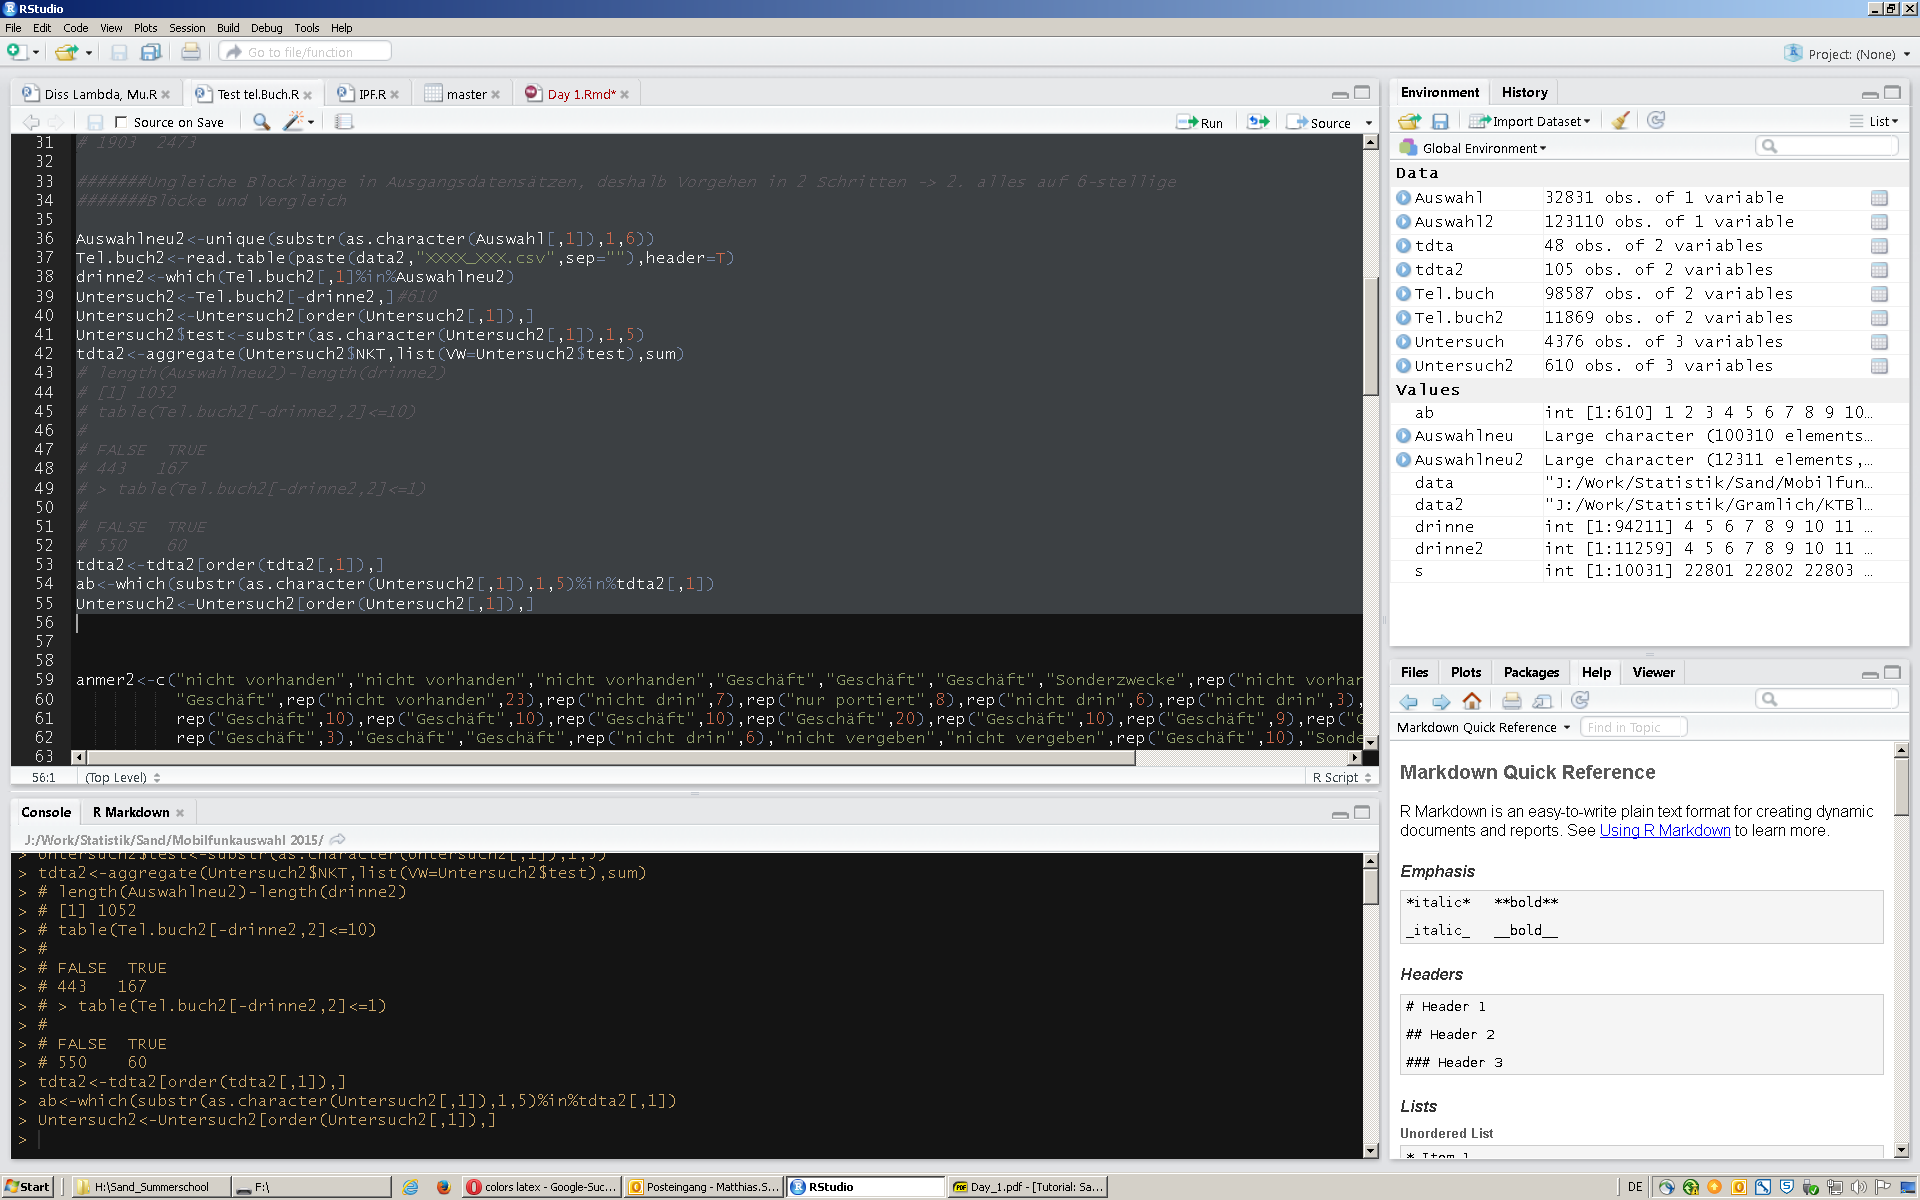
\includegraphics[width=\linewidth, height=6cm]{../figure/RStudio.png}
\vspace{.5cm}
\begin{center}
\url{https://www.rstudio.com}
\end{center}
\end{frame}
%%%%%%%%%%%%%%%%%%%%%%%%%%%%%%%%%%%%%%%%%%%%%%%%%%%%%%%%%%%%%%%%%%%%
\begin{frame}[fragile]{Basic R Commands}
%\frametitle{\vspace{-.05cm}\begin{center}\footnotesize{Basic R Commands}\end{center}}
\begin{itemize}
\item \R{<-}  assignment operator
\item \R{\#} can be used to comment your script
\item \R{x<-rnorm(10,0,1)}  creates a vector with ten standardnormal-distributed values
\item \R{mean(x)} calculates the mean of variable \R{x}; \R{length(x)} returns the number of observations in \R{x}
\end{itemize}
\begin{Schunk}
\begin{Sinput}
 mean(x)
\end{Sinput}
\begin{Soutput}
[1] -0.6266963
\end{Soutput}
\begin{Sinput}
 length(x)
\end{Sinput}
\begin{Soutput}
[1] 10
\end{Soutput}
\end{Schunk}
\end{frame}
%%%%%%%%%%%%%%%%%%%%%%%%%%%%%%%%%%%%%%%%%%%%%%%%%%%%%%%%%%%%%%%%%%%%%
\begin{frame}[fragile]{Getting Help}
%\frametitle{\vspace{-.05cm}\begin{center}\footnotesize{Getting Help}\end{center}}
\begin{itemize}
\item \R{?\emph{command}}
\end{itemize}
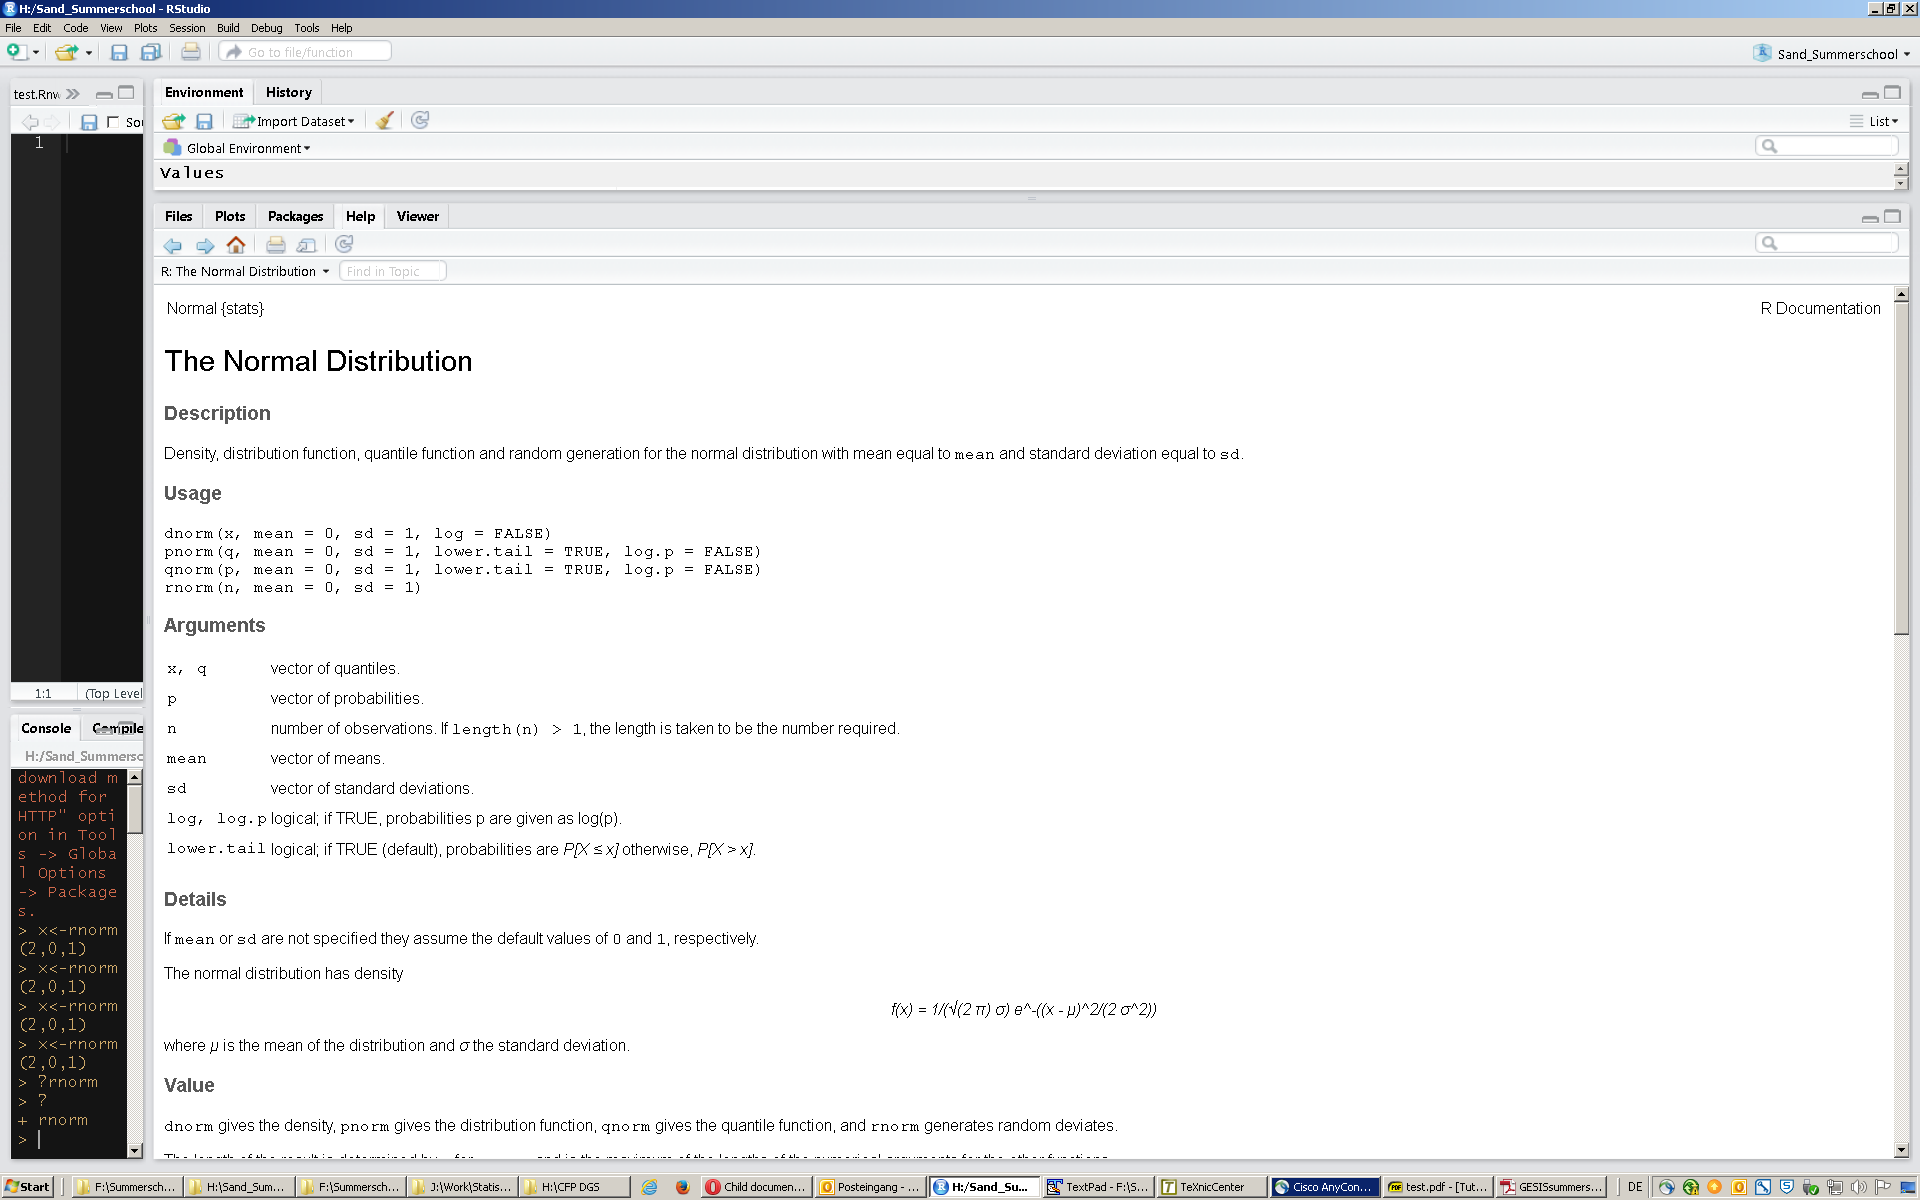
\includegraphics[width=\textwidth, height=4cm]{../figure/rhlep.png}
\begin{itemize}
\item \href{https://cran.r-project.org}{CRAN}
\item \href{http://www.statmethods.net}{Quick-R}
\item \href{http://stackoverflow.com/questions/tagged/r}{stackoverflow.com}
\end{itemize}

\end{frame}
%%%%%%%%%%%%%%%%%%%%%%%%%%%%%%%%%%%%%%%%%%%%%%%%%%%%%%%%%%%%%%%%%%%%%%%%%
\begin{frame}[fragile]{Types of Data}
%\frametitle{\vspace{-.05cm}\begin{center}\footnotesize{Types of Data}\end{center}}
\begin{tabular}{l l}
numeric & \R{x<-c(1,2)}\\
logical & \R{x<-c(T,F)}\\
character & \R{x<-c("A","B")}\\
factor & \R{x<-as.factor(c("White","Black"))}\\
\end{tabular}\\
\vspace{.25cm}
\R{str()} returns the type of your data
\begin{Schunk}
\begin{Sinput}
 x<-as.factor(c("White","Black"))
 str(x)
\end{Sinput}
\begin{Soutput}
 Factor w/ 2 levels "Black","White": 2 1
\end{Soutput}
\end{Schunk}
\end{frame}
%%%%%%%%%%%%%%%%%%%%%%%%%%%%%%%%%%%%%%%%%%%%%%%%%%%%%%%%%%%%%%%%%%%%%%%%
\begin{frame}[fragile]{Indexing I}
%\frametitle{\vspace{-.05cm}\begin{center}\footnotesize{Indexing I}\end{center}}
\begin{center}
\textbf{Indexing a Vector:}
\end{center}
\begin{Schunk}
\begin{Sinput}
 A1<-c(1,2,3,4)
 A1[1]
\end{Sinput}
\begin{Soutput}
[1] 1
\end{Soutput}
\begin{Sinput}
 A1[1:3]
\end{Sinput}
\begin{Soutput}
[1] 1 2 3
\end{Soutput}
\begin{Sinput}
 A1[-2]
\end{Sinput}
\begin{Soutput}
[1] 1 3 4
\end{Soutput}
\end{Schunk}
\end{frame}
%%%%%%%%%%%%%%%%%%%%%%%%%%%%%%%%%%%%%%%%%%%%%%%%%%%%%%%%%%%%%%%%%%%%%%%%%%
\begin{frame}[fragile]{Indexing II}
%\frametitle{\vspace{-.05cm}\begin{center}\footnotesize{Indexing II}\end{center}}
\begin{center}
\textbf{Indexing a data frame:}
\end{center}
\begin{Schunk}
\begin{Sinput}
 A2<-4:1
 AA<-cbind(A1,A2)
 AA[1,]
\end{Sinput}
\begin{Soutput}
A1 A2 
 1  4 
\end{Soutput}
\begin{Sinput}
 AA[,1]
\end{Sinput}
\begin{Soutput}
[1] 1 2 3 4
\end{Soutput}
\begin{Sinput}
 AA[1:3,2]
\end{Sinput}
\begin{Soutput}
[1] 4 3 2
\end{Soutput}
\begin{Sinput}
 AA[,-1]
\end{Sinput}
\begin{Soutput}
[1] 4 3 2 1
\end{Soutput}
\end{Schunk}
\end{frame}
%%%%%%%%%%%%%%%%%%%%%%%%%%%%%%%%%%%%%%%%%%%%%%%%%%%%%%%%%%%%%%%%%%%%%%%%%%
\begin{frame}[fragile]{Indexing III}
%\frametitle{\vspace{-.05cm}\begin{center}\footnotesize{Indexing III}\end{center}}
\begin{center}
\textbf{Indexing an array}
\end{center}
\begin{scriptsize}
\begin{Schunk}
\begin{Sinput}
 A3<-array(1:8,c(2,2,2))
 A3
\end{Sinput}
\begin{Soutput}
, , 1

     [,1] [,2]
[1,]    1    3
[2,]    2    4

, , 2

     [,1] [,2]
[1,]    5    7
[2,]    6    8
\end{Soutput}
\begin{Sinput}
 A3[,,2]
\end{Sinput}
\begin{Soutput}
     [,1] [,2]
[1,]    5    7
[2,]    6    8
\end{Soutput}
\end{Schunk}
\end{scriptsize}
\end{frame}
%%%%%%%%%%%%%%%%%%%%%%%%%%%%%%%%%%%%%%%%%%%%%%%%%%%%%%%%%%%%%%%%%%%%%%%%%%
\begin{frame}[fragile]{Indexing IV}
%\frametitle{\vspace{-.05cm}\begin{center}\footnotesize{Indexing IV}\end{center}}
\begin{center}
\textbf{Indexing a list}
\end{center}
\begin{Schunk}
\begin{Sinput}
 A4<-list(A1,c("Summer","Winter"))
 A4
\end{Sinput}
\begin{Soutput}
[[1]]
[1] 1 2 3 4

[[2]]
[1] "Summer" "Winter"
\end{Soutput}
\begin{Sinput}
 A4[[1]]
\end{Sinput}
\begin{Soutput}
[1] 1 2 3 4
\end{Soutput}
\end{Schunk}
\end{frame}
%%%%%%%%%%%%%%%%%%%%%%%%%%%%%%%%%%%%%%%%%%%%%%%%%%%%%%%%%%%%%%%%%%%%%%%%%%
\begin{frame}[fragile]{Sequences}
%\frametitle{\vspace{-.05cm}\begin{center}\footnotesize{Sequences}\end{center}}
\begin{Schunk}
\begin{Sinput}
 1:5
\end{Sinput}
\begin{Soutput}
[1] 1 2 3 4 5
\end{Soutput}
\begin{Sinput}
 rep("A",times=10)
\end{Sinput}
\begin{Soutput}
 [1] "A" "A" "A" "A" "A" "A" "A" "A" "A" "A"
\end{Soutput}
\begin{Sinput}
 rep(1:3,times=2,each=3)
\end{Sinput}
\begin{Soutput}
 [1] 1 1 1 2 2 2 3 3 3 1 1 1 2 2 2 3 3 3
\end{Soutput}
\begin{Sinput}
 seq(-5,5,by=2.5)
\end{Sinput}
\begin{Soutput}
[1] -5.0 -2.5  0.0  2.5  5.0
\end{Soutput}
\end{Schunk}
\end{frame}
%%%%%%%%%%%%%%%%%%%%%%%%%%%%%%%%%%%%%%%%%%%%%%%%%%%%%%%%%%%%%%%%%%%%%%%%%%%%
\begin{frame}[fragile]{Random Numbers}
%\frametitle{\vspace{-.05cm}\begin{center}\footnotesize{Random Numbers}\end{center}}
\begin{center}
\begin{tabular}{l|l|l}
\textbf{Function } & \textbf{Distribution} & \textbf{Important parameter} \\
\hline
\hline
\R{runif()} & Uniform distribution & n, min, max\\
\hline
\R{rnorm()} & Normal distribution & n, mean, sd \\
\hline
\R{rpois()} & Poisson distribution & n, lambda\\
\hline 
... & ... & ... \\
\end{tabular}
\end{center}
\end{frame}

%%%%%%%%%%%%%%%%%%%%%%%%%%%%%%%%%%%%%%%%%%%%%%%%%%%%%%%%%%%%%%%%%%%%%%%%%%
\begin{frame}[fragile]{Important Functions} {of the \{base\}-Package}
%\frametitle{\vspace{-.05cm}\begin{center}\footnotesize{Important Functions of the \{base\}-Package}\end{center}}
\begin{center}
\renewcommand{\arraystretch}{.75}
\begin{tabular}{lll}
Function & Meaning & Example \\
\hline
\R{length()} & Length & \R{length(x)}\\
\R{max()} & Maximum & \R{max(x)}\\
\R{min()} & Minimum & \R{min(x)}\\
\R{sd()} & Standard deviation & \R{sd(x)}\\
\R{var()} & Variance & \R{var(x)}\\
\R{mean()} & Mean & \R{mean(x)} \\
\R{median()} & Median & \R{median(x)} \\
&& \\
\multicolumn{3}{c}{These functions do only need one argument}\\
\multicolumn{3}{c}{Other functions need to be specified by further arguments:}\\
&& \\
\R{quantile()} & 90\% Quantile & \R{quantile(x,.9)}\\ 
\R{sample()} & Draw a sample & \R{sample(x,1)}\\
\end{tabular}
\end{center}
\begin{itemize}
\pause\item \R{R} is a modular program with many functions included in basic \R{R}
\pause\item more specific functions are embedded in further packages
\end{itemize}
\end{frame}


%%%%%%%%%%%%%%%%%%%%%%%%%%%%%%%%%%%%%%%%%%%%%%%%%%%%%%%%%%%%%%%%%%%%%%%%%%
\begin{frame}[fragile]{Installing and Loading Packages}
%\frametitle{\vspace{-.05cm}\begin{center}\footnotesize{Installing and Loading Packages}\end{center}}
\R{install.package("sampling")}\\
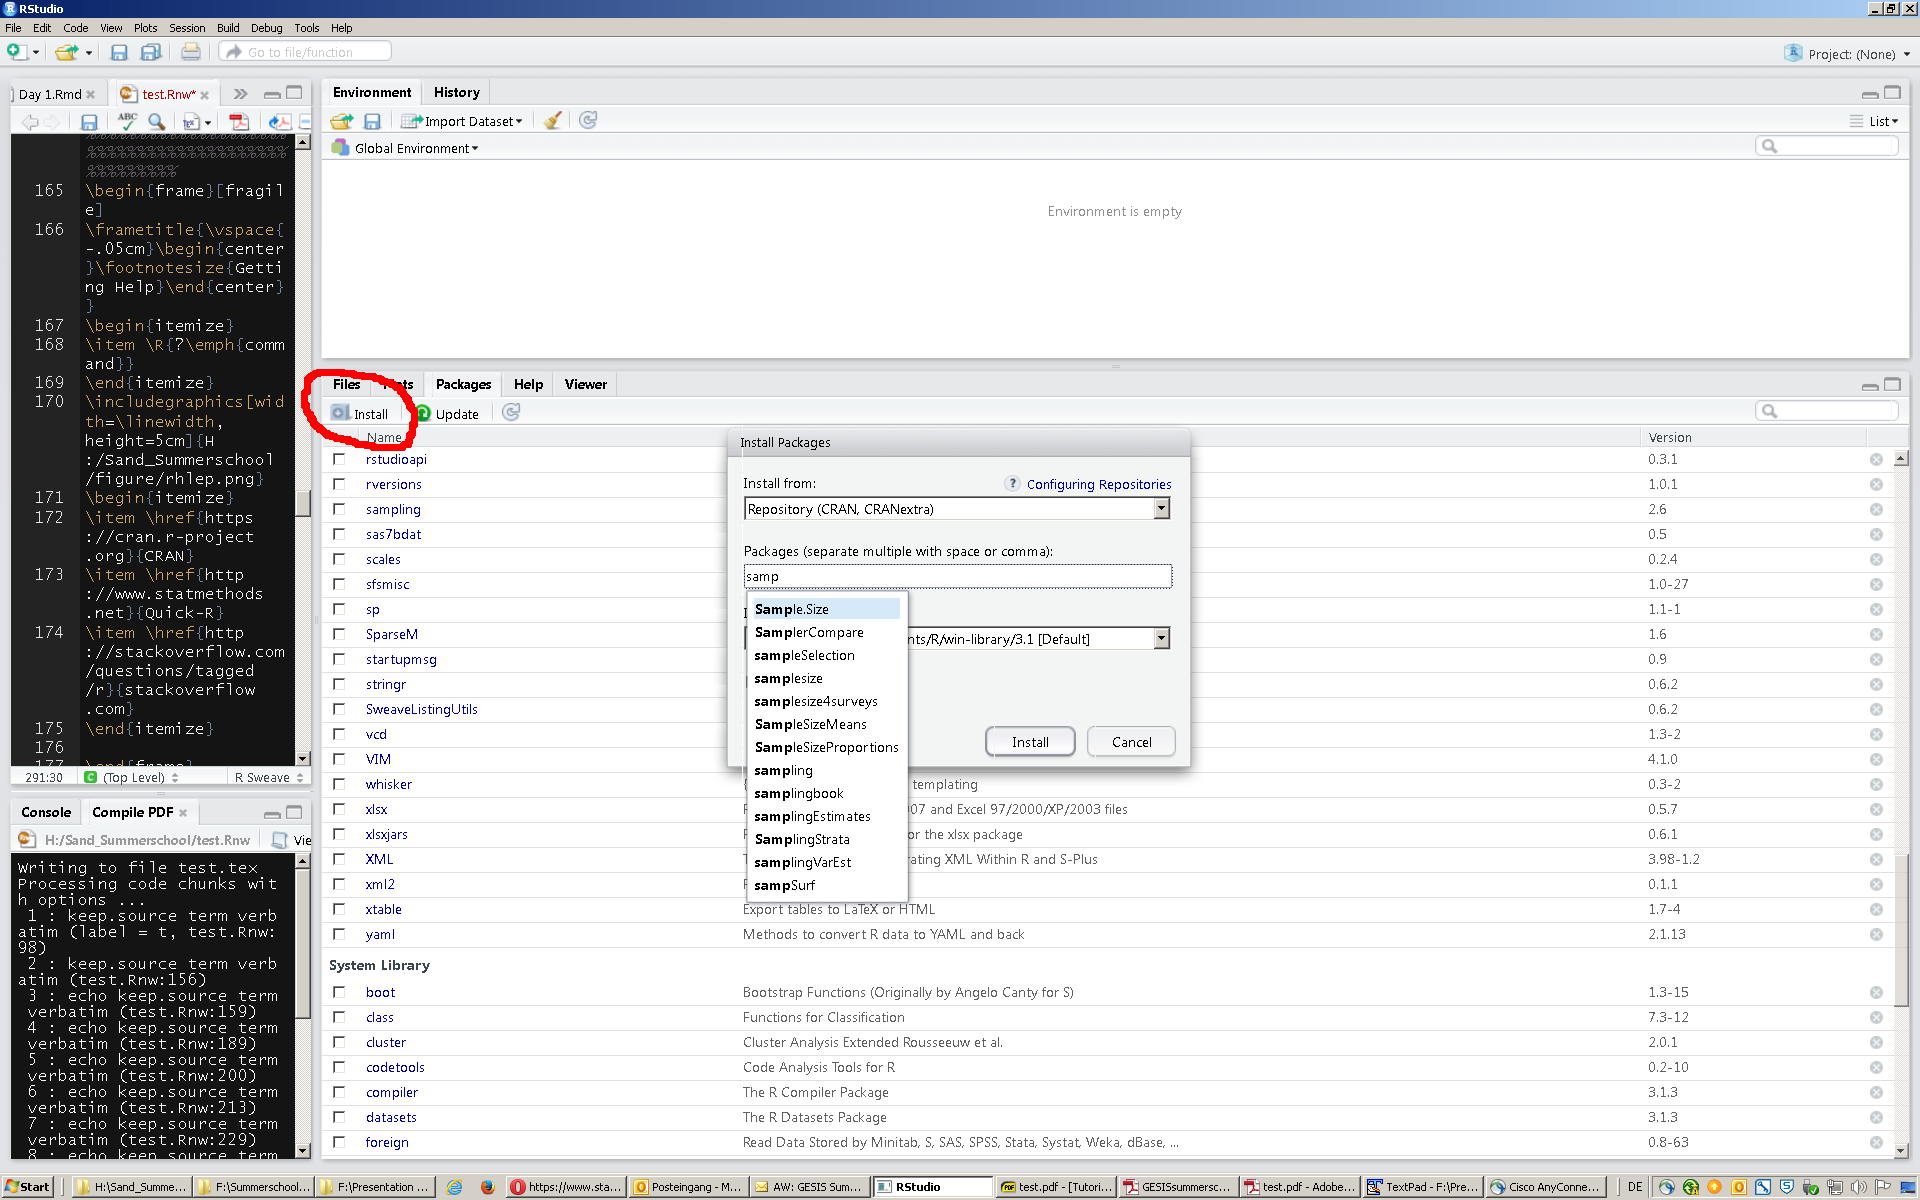
\includegraphics[width=\linewidth, height=5cm]{../figure/Rpackages.png}
\vspace{.25cm}
\R{library(sampling)} \emph{or} \R{require(sampling)}
\end{frame}
%%%%%%%%%%%%%%%%%%%%%%%%%%%%%%%%%%%%%%%%%%%%%%%%%%%%%%%%%%%%%%%%%%%%%%%%%%
\begin{frame}[fragile]{Useful Packages}
%\frametitle{\vspace{-.05cm}\begin{center}\footnotesize{Useful Packages}\end{center}}
\renewcommand{\arraystretch}{1}
\begin{tabular}{l|l}
Library & Subject\\
\hline
\R{foreign} & reading and writing of data in\\ 
& numerous formats (e.g. \emph{.dta}, \emph{.sav})\\
\R{sampling} & drawing and weighting samples\\
\R{survey} & analysis of complex survey samples\\
\R{xlsx} & read and write data in Excell-Format\\
\R{xtable} & export tables to LaTex and HTML\\
\R{mice} & multiple imputation by chain equation\\
\R{reshape} & alter structure of datasets\\
\R{car} & applied regressions\\
\R{VIM} & visualization and imputation of Missing Values\\
\R{lattice} & high-level data visualization\\
\R{ggplot2} & grammar for graphics in \R{R}\\
\end{tabular}
\end{frame}
%%%%%%%%%%%%%%%%%%%%%%%%%%%%%%%%%%%%%%%%%%%%%%%%%%%%%%%%%%%%%%%%%%%%%%%%%%
\begin{frame}[fragile]{Basic Graphics}
%\frametitle{\vspace{-.05cm}\begin{center}\footnotesize{Basic Graphics}\end{center}}

\begin{columns}
\begin{column}{.5\textwidth}
\begin{Schunk}
\begin{Sinput}
 set.seed(42)
 x <- rnorm(1000,0,1)
 plot(x)
\end{Sinput}
\end{Schunk}
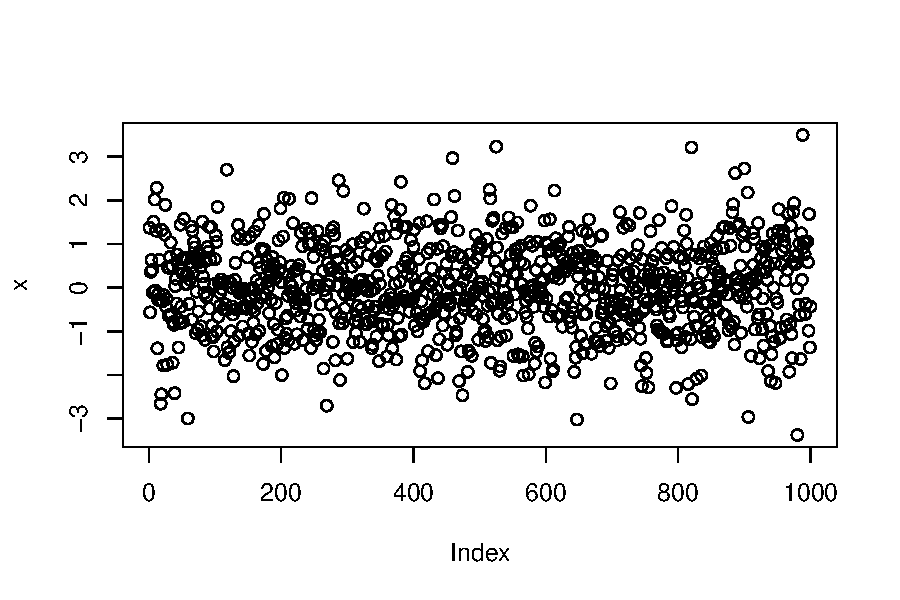
\includegraphics{Day1-010}
\end{column}
\vspace{.25cm}
\begin{column}{.5\textwidth}

\R{set.seed()} is used to specify a starting point

\begin{Schunk}
\begin{Sinput}
 hist(x)
\end{Sinput}
\end{Schunk}
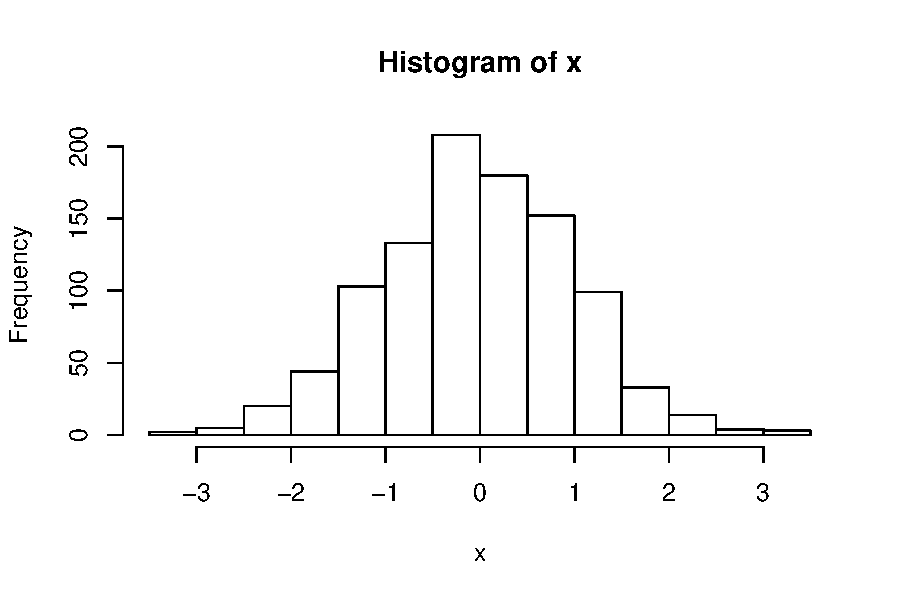
\includegraphics{Day1-011}
\end{column}
\end{columns}
\begin{itemize}
\item[$\Rightarrow$] we will use \emph{42} as seed-value for future exercises to obtain comparable results
\end{itemize}
\end{frame}
%%%%%%%%%%%%%%%%%%%%%%%%%%%%%%%%%%%%%%%%%%%%%%%%%%%%%%%%%%%%%%%%%%%%%%%%%%
\begin{frame}[fragile]{The Basic \R{sample} Function}
%\frametitle{\vspace{-.05cm}\begin{center}\footnotesize{The Basic \R{sample} Function}\end{center}}
\begin{center}
\pgfdeclareimage[width=.6\textwidth]{SampleHelp}{../figure/SampleHelp.PNG}
\pgfuseimage{SampleHelp}

\pgfdeclareimage[width=.6\textwidth]{SampleWhat}{../figure/SampleWhat2.PNG}
\pgfdeclareimage[width=.6\textwidth]{SampleHow}{../figure/SampleHow.PNG}
\pgfdeclareimage[width=.6\textwidth]{SampleReplacement}{../figure/SampleReplacement.PNG}

\pgfuseimage<1>{SampleWhat}
\pgfuseimage<2>{SampleHow}
\pgfuseimage<3>{SampleReplacement}

\end{center}
\end{frame}
%%%%%%%%%%%%%%%%%%%%%%%%%%%%%%%%%%%%%%%%%%%%%%%%%%%%%%%%%%%%%%%%%%%%%%%%%%
\begin{frame}[fragile]{Simple Example on Sampling}
%\frametitle{\vspace{-.05cm}\begin{center}\footnotesize{Simple Example on Sampling}\end{center}}
\begin{footnotesize}
\begin{Schunk}
\begin{Sinput}
 id <- 1:10000
 set.seed(42)
 education <- sample(c("none","low","average","high"),10000, 
+                     replace = T,prob = c(.072,.356,.289,.283))
 gender <- sample(c("male","female"),10000,
+                  replace = T,prob = c(.488,.512))
 iq <- rnorm(10000,100,20)
 my.pop <- data.frame(id,gender,education,iq)
 head(my.pop)
\end{Sinput}
\begin{Soutput}
  id gender education        iq
1  1   male      high 123.26218
2  2   male      none  96.19531
3  3   male       low  94.21088
4  4 female      high  92.02308
5  5   male   average 114.18485
6  6   male   average  67.54705
\end{Soutput}
\end{Schunk}
\end{footnotesize}
\end{frame}
%%%%%%%%%%%%%%%%%%%%%%%%%%%%%%%%%%%%%%%%%%%%%%%%%%%%%%%%%%%%%%%%%%%%%%%%55
\begin{frame}[fragile]{Simple Example on Sampling}{Summary of the dataset}
%\frametitle{\vspace{-.05cm}\begin{center}\footnotesize{Simple Example on Sampling}\\ \scriptsize{Summary of the dataset}\end{center}}
\begin{footnotesize}
\begin{Schunk}
\begin{Sinput}
 summary(my.pop)
\end{Sinput}
\begin{Soutput}
       id           gender       education          iq        
 Min.   :    1   female:5125   average:2851   Min.   : 30.93  
 1st Qu.: 2501   male  :4875   high   :2820   1st Qu.: 86.50  
 Median : 5000                 low    :3588   Median :100.08  
 Mean   : 5000                 none   : 741   Mean   :100.02  
 3rd Qu.: 7500                                3rd Qu.:113.60  
 Max.   :10000                                Max.   :173.26  
\end{Soutput}
\begin{Sinput}
 prop.table(table(my.pop$gender,my.pop$education))
\end{Sinput}
\begin{Soutput}
         average   high    low   none
  female  0.1449 0.1465 0.1844 0.0367
  male    0.1402 0.1355 0.1744 0.0374
\end{Soutput}
\begin{Sinput}
 var(my.pop$iq)*(nrow(my.pop)-1)/nrow(my.pop)
\end{Sinput}
\begin{Soutput}
[1] 406.1684
\end{Soutput}
\end{Schunk}
\begin{itemize}\footnotesize{
\item[$\Rightarrow$]$\sigma^2$}
\end{itemize}
\end{footnotesize}
\end{frame}
%%%%%%%%%%%%%%%%%%%%%%%%%%%%%%%%%%%%%%%%%%%%%%%%%%%%%%%%%%%%%%%%%%%%%%%%%%%%
\begin{frame}[fragile]{Simple Example on Sampling}
%\frametitle{\vspace{-.05cm}\begin{center}\footnotesize{Simple Example on Sampling}\end{center}}
\footnotesize{
\begin{Schunk}
\begin{Sinput}
 set.seed(42)
 s.SRS <- sample(1:nrow(my.pop),500,replace=T)
 s.SRSWOR <- sample(1:nrow(my.pop),500,replace=F)
 my.samp.SRS <- my.pop[s.SRS,]
 my.samp.SRSWOR <- my.pop[s.SRSWOR,]
 summary(my.samp.SRS)
\end{Sinput}
\begin{Soutput}
       id          gender      education         iq        
 Min.   :   3   female:257   average:132   Min.   : 45.95  
 1st Qu.:2322   male  :243   high   :134   1st Qu.: 85.38  
 Median :4804                low    :192   Median :100.00  
 Mean   :4896                none   : 42   Mean   : 99.60  
 3rd Qu.:7434                              3rd Qu.:113.20  
 Max.   :9966                              Max.   :165.63  
\end{Soutput}
\begin{Sinput}
 nrow(unique(my.samp.SRS))
\end{Sinput}
\begin{Soutput}
[1] 487
\end{Soutput}
\end{Schunk}
}
\end{frame}
%%%%%%%%%%%%%%%%%%%%%%%%%%%%%%%%%%%%%%%%%%%%%%%%%%%%%%%%%%%%%%%%%%%%%%%%%
\begin{frame}[fragile]{Simple Example on Sampling}
%\frametitle{\vspace{-.05cm}\begin{center}\footnotesize{Simple Example on Sampling}\end{center}}
\begin{Schunk}
\begin{Sinput}
 plot(density(my.pop$iq),main = "My first density plot"
+      , xlab = "IQ")
 abline(v=mean(my.pop$iq), col = "black")
 lines(density(my.samp.SRS$iq),col = "red",lwd=2)
 lines(density(my.samp.SRSWOR$iq),col = "blue",lwd=2)
\end{Sinput}
\end{Schunk}
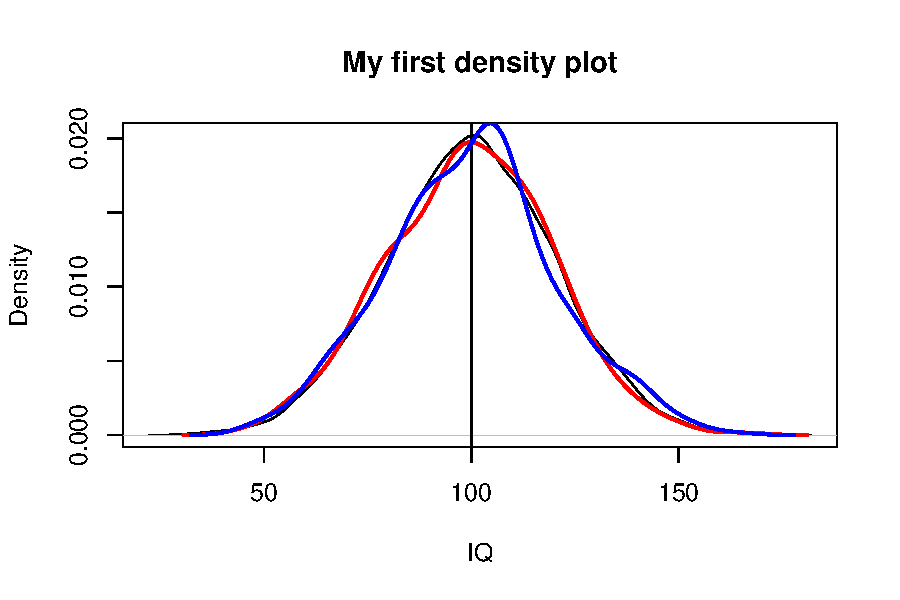
\includegraphics{Day1-015}
\end{frame}
%%%%%%%%%%%%%%%%%%%%%%%%%%%%%%%%%%%%%%%%%%%%%%%%%%%%%%%%%%%%%%%%%%%%%%%%%
\begin{frame}[fragile]{Simple Example on Sampling}{the sampling package}
%\frametitle{\vspace{-.05cm}\begin{center}\footnotesize{Simple Example on Sampling}\\ \scriptsize{the sampling package}\end{center}}
\begin{Schunk}
\begin{Sinput}
 library(sampling)
 set.seed(42)
 s.SRS1 <- srswr(500,nrow(my.pop))
 s.SRSWOR1 <- srswor(500,nrow(my.pop)) 
 my.samp.SRS1 <- rbind(my.pop[s.SRS1!=0,]
+                       ,my.pop[s.SRS1>1,])
 my.samp.SRSWOR1 <- my.pop[s.SRSWOR1==1,]
\end{Sinput}
\end{Schunk}
\end{frame}
%%%%%%%%%%%%%%%%%%%%%%%%%%%%%%%%%%%%%%%%%%%%%%%%%%%%%%%%%%%%%%%%%%%%%%%%%%%%
\begin{frame}[fragile]{Simple Example on Sampling}{the sampling package}
%\frametitle{\vspace{-.05cm}\begin{center}\footnotesize{Simple Example on Sampling}\\ \scriptsize{the sampling package}\end{center}}
\begin{Schunk}
\begin{Sinput}
 par(mfrow=c(1,2))
\end{Sinput}
\end{Schunk}
\begin{minipage}{5.5cm}
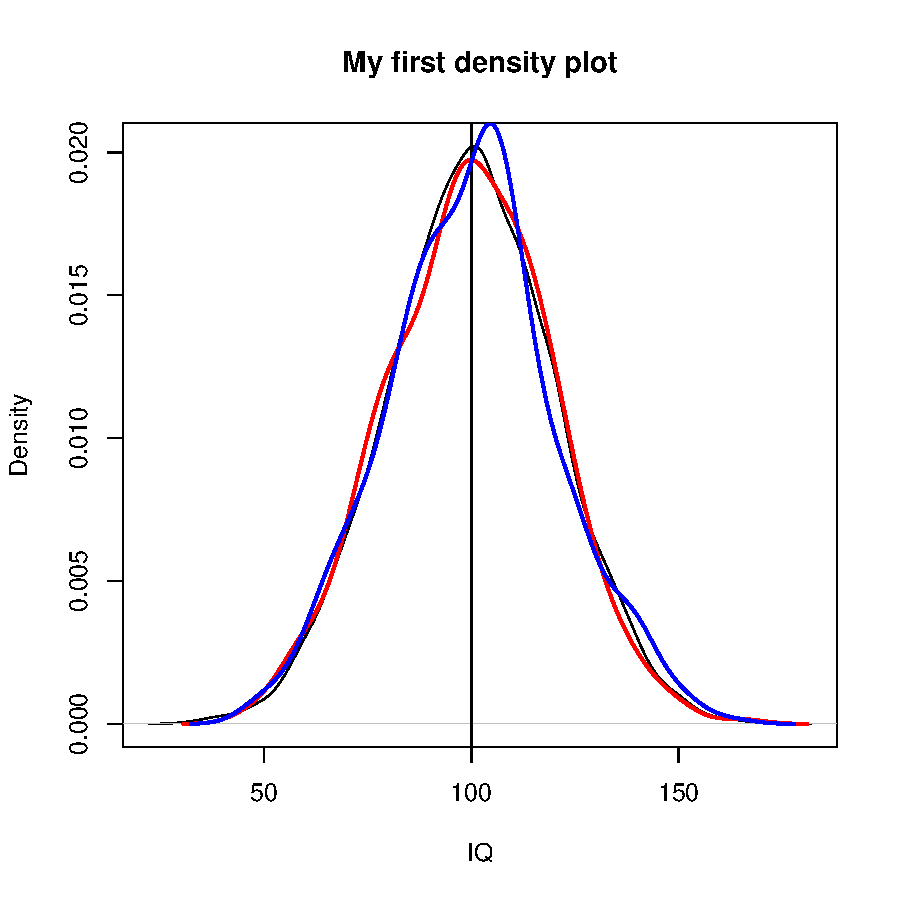
\includegraphics{Day1-018}
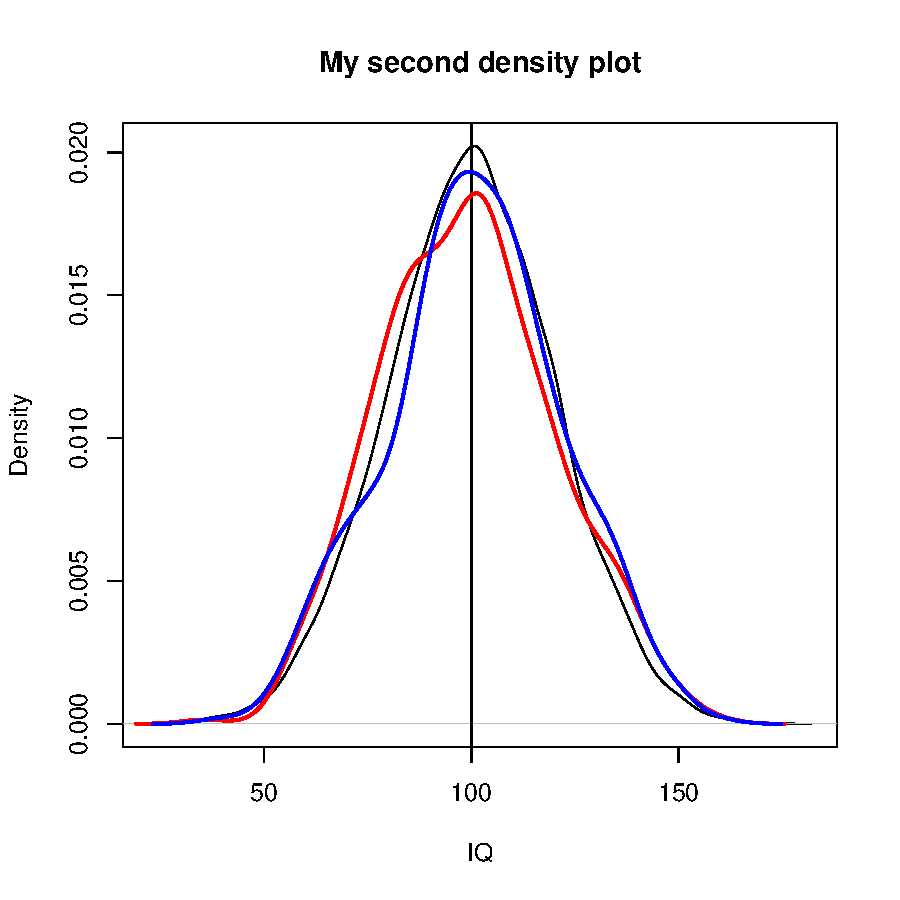
\includegraphics{Day1-019}
\end{minipage}
\begin{Schunk}
\begin{Sinput}
 dev.off()
\end{Sinput}
\end{Schunk}
\begin{itemize}
\pause\item should yield same results
\item[$\Rightarrow$] routine differs in "starting point"
\end{itemize}
\end{frame}
%%%%%%%%%%%%%%%%%%%%%%%%%%%%%%%%%%%%%%%%%%%%%%%%%%%%%%%%%%%%%%%%%%%%%%%%%%%
\begin{frame}[fragile]{Working Directory and Workspace}
%\frametitle{\vspace{-.05cm}\begin{center}\footnotesize{Working Directory and Workspace}\end{center}}
\footnotesize{
\begin{center}
\textbf{Declaring a working directory}\\
\end{center}
\R{path<-"H:/Sand\_ Summerschool/Data Day1/"\\
setwd(path)}}
\begin{itemize}
\footnotesize{
\item It is always useful to define and set your working directory at the beginning of each script
\item \R{getwd()} displays you your current working directory
\item \R{dir()} shows you all objects in a specific directory
\item \R{ls()} lists all objects in your workspace
\item \R{rm()} removes a object from your workspace
}
\end{itemize}
\footnotesize{
Example:\\
\begin{Schunk}
\begin{Sinput}
 rm(list = ls())
\end{Sinput}
\end{Schunk}
}

\end{frame}





%%%%%%%%%%%%%%%%%%%%%%%%%%%%%%%%%%%%%%%%%%%%%%%%%%%%%%%%%%%%%%%%%%%%%%%%%%%

\begin{frame}[fragile]{Reading and Writing Data}
%\frametitle{\vspace{-.05cm}\begin{center}\footnotesize{Reading and Writing Data}\end{center}}
\footnotesize{
\begin{center}
\textbf{Writing/ saving data and results}\\
\end{center}
\R{write.table(my.pop,"Synthetic Data Day1.csv",\\
            row.names = F, quote = F, dec = ".",sep = ",")}\\ 
            \textbf{OR:}\\
\R{save(my.samp.SRS,s.SRS,my.samp.SRSWOR1,file = "Day1.Rdata")}\\
\begin{itemize}
\item[$\Rightarrow$] See also: \R{write.csv} and \R{write.csv2} (\R{sep = }";")
\end{itemize}
\begin{center}
\textbf{Reading/ loading data and results}\\
\end{center}
\R{d1 <- read.table("Synthetic Data Day1.csv",\\
            header = F, dec = ".",sep = ",")}\\
            \textbf{OR:}\\
\R{load("Day1.Rdata")}}

\end{frame}
%%%%%%%%%%%%%%%%%%%%%%%%%%%%%%%%%%%%%%%%%%%%%%%%%%%%%%%%%%%%%%%%%%%%%%%%%%%
\begin{frame}[fragile]{Exercise 1}
%\frametitle{\vspace{-.05cm}\begin{center}\footnotesize{Exercise 1}\end{center}}
\begin{exampleblock}{Sample sizes}
\begin{enumerate}
\item Generate 1000 numbers from a exponential distribution
\item Draw three samples(n1=2,n2=10,n3=100)
\item Plot the density and add the means of the three samples as vertical lines
\end{enumerate}
\end{exampleblock}
\end{frame}
%%%%%%%%%%%%%%%%%%%%%%%%%%%%%%%%%%%%%%%%%%%%%%%%%%%%%{Exercise 2}%%%%%%%%%%%%%%%%%%%%%%
\begin{frame}[fragile]{Exercise 2}
%\frametitle{\vspace{-.05cm}\begin{center}\footnotesize{Exercise 2}\end{center}}
\begin{exampleblock}{Belgian municipalities/ variance decomposition}
\begin{enumerate}\footnotesize{
\item Load the dataset "belgianmunicipalities" from the \R{sample}-package using the \R{data()}-command 
\item Inspect the structure of the dataset
\item Calculate mean and variance of the variable \R{averageincome} 
\item Calculate the mean of each province for that variable, plot your results and add the mean of \alert{3} 
\item Recalculate the mean of \R{averageincome} based on the means by province and compare your results
\item Make a boxplot of the variable \R{averageincome} for each province
\item Calculate the variance of \R{averageincome} using variance decomposition and compare it with \alert{3}
\begin{itemize}
\item[$\Rightarrow$]\footnotesize{ Advice: consider the dataset as the aggregates for the whole population and use the formula for the population variance}
\end{itemize}
}
\end{enumerate}
\end{exampleblock}

\end{frame}



\end{document}
